%%% -*-LaTeX-*-

\chapter[Memory-Efficient Mixed-Precision Implementations for Robust Explicit Model Predictive Control]{Memory-Efficient Mixed-Precision Implementations for Robust\\Explicit Model Predictive\\Control}
\label{sec:emsoft}
Reprinted from Proceedings of the 19th International Conference on Embedded Software (EMSOFT), ACM Trans. Embed. Comput. Syst., Vol. 18, No. 5s, Article 100, October 2019: "Memory-Efficient Mixed-Precision Implementations for Robust Explicit Model Predictive Control" by Mahmoud Salamati, Rocco Salvia, Eva Darulova, Sadegh Soudjani, and Rupak Majumdar. Reprinted by permission.\\
https://doi.org/10.1145/3358223

\setupuuchapterbib

\uudummysection {Introduction}                              {1}
\uudummysection {Overview}                            		{3}
\uudummyfigure   {Overview of the proposed memory-efficient robust EMPC control design.}          					{3}
\uudummyfigure   {(a) Inverted pendulum; (b) 2D plot of polyhedral partitions for an EMPC for the inverted pendulum.}          					{4}
\uudummysection {Background}       							{5}
\uudummysubsection {Robust Explicit MPC}       				{5}
\uudummyfigure {Structure of an explicit MPC controller}          					{6}
\uudummysubsection {Finite-Precision Implementation}       	{6}
\uudummysection {Error Analysis}                      		{7}
\uudummysubsection {Incorrect Region Selection}             {7}
\uudummysubsection {Approximate Control Output}             {9}
\uudummysubsection {Implementation}             			{9}
\uudummysection {Controller Synthesis}						{9}
\uudummyfigure {Algorithm for designing memory-efficient robust EMPC controller}          					{10}
\uudummysubsection {Implementation}             			{11}
\uudummysection {Experimental Results}                      {11}
\uudummysubsection {End-to-End Robust Controller}           {11}

\uudummytable {Inverted Pendulum and Aircraft. Memory requirements in number of bits for storing F, G and H, K for uniform 32 bit precision (Uni32), uniform custom precision (Uni, word length chosen in parentheses) and mixed precision (Mix), for different values of $\Delta$ a$\epsilon_{Q}$. \%32vsU is the percentage of memory saved using Uni compared to the baseline Uni32, and \%UvsM is the percentage of memory saved using Mix compared to Uni.}          					{12}

\uudummytable {Double Integrator. N is the prediction horizon in RMPC, time gives the execution time in minutes, Regs is the number of regions of the controller with Hyps hyperplanes. Uni32 is the total number of bits when all operations are in 32 bits, Uni the minimal uniform precision required, Mix is mixed-precision, \%32vU and \%UvM give the improvements of uniform and mixed precisions.}          					{12}

\uudummysubsection {Scalability}           					{13}
\uudummysection {Related Work}       						{14}
\uudummysection {Conclusion}                      			{15}
\uudummysection {References}                              	{15}

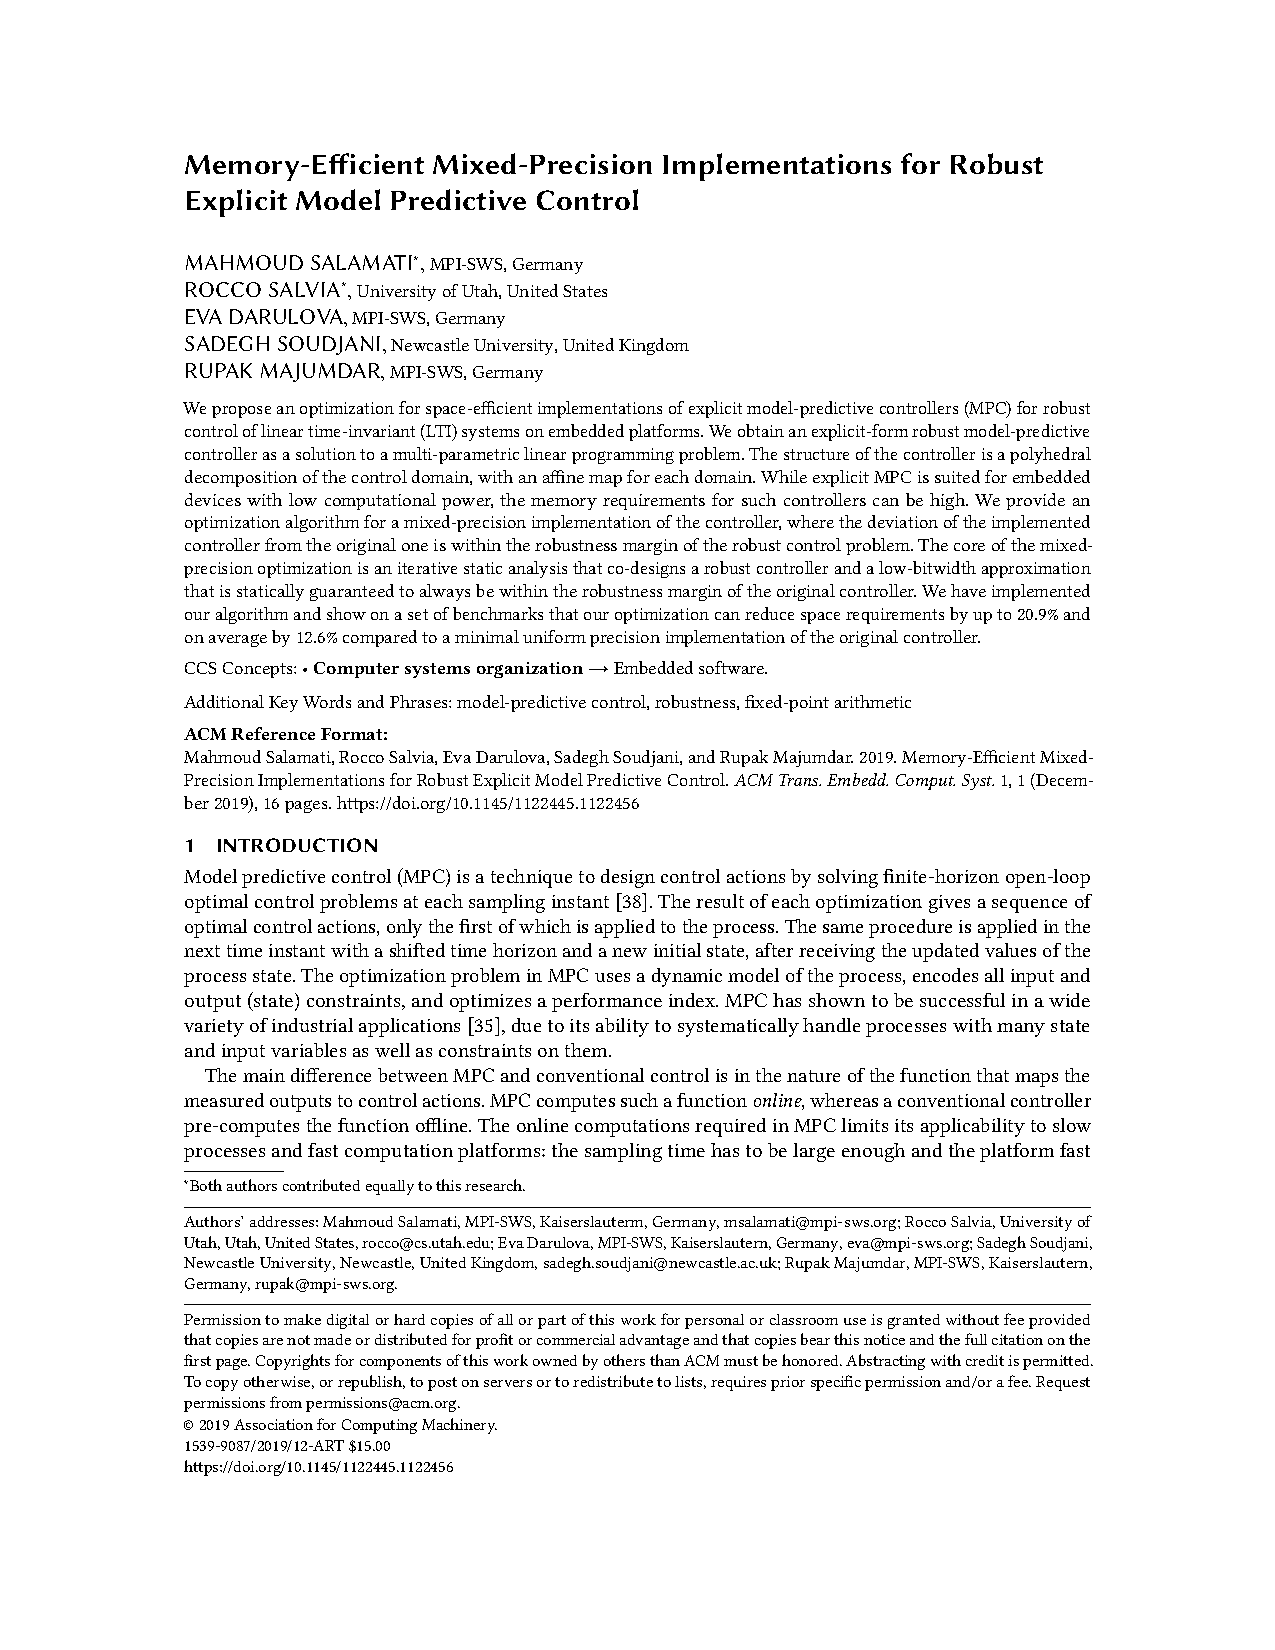
\includepdf[
	pages = -,          % want all document pages
	scale = 0.95,       % adjust to fit thesis page box
	pagecommand = {\pagestyle{plain}} % bare page numbers
]{emsoft/main.pdf}
